\documentclass{article}

\usepackage{fancyhdr} % Required for custom headers
\usepackage{lastpage} % Required to determine the last page for the footer
\usepackage{extramarks} % Required for headers and footers
\usepackage[usenames,dvipsnames]{color} % Required for custom colors
\usepackage{graphicx} % Required to insert images
\usepackage{listings} % Required for insertion of code
\usepackage{courier} % Required for the courier font
\usepackage{caption}
\usepackage{multirow}
\usepackage{subcaption}
\renewcommand{\_}{\char`_}

% Margins
\topmargin=-0.45in
\evensidemargin=0in
\oddsidemargin=0in
\textwidth=6.5in
\textheight=9.0in
\headsep=0.25in

\linespread{1.1} % Line spacing

\lstset{language=C,
                basicstyle=\ttfamily,
                keywordstyle=\color{blue}\ttfamily,
                stringstyle=\color{red}\ttfamily,
                commentstyle=\color{Plum}\ttfamily,
                morecomment=[l][\color{magenta}]{\#}
}


% Set up the header and footer
\pagestyle{fancy}
\lhead{Group 18} % Top left header
\chead{Task 1: Scheduling} % Top center head
\rhead{\firstxmark} % Top right header
\lfoot{\lastxmark} % Bottom left footer
\rfoot{Page\ \thepage\ of\ \protect\pageref{LastPage}} % Bottom right footer
\renewcommand\headrulewidth{0.4pt} % Size of the header rule
\renewcommand\footrulewidth{0.4pt} % Size of the footer rule

\setlength\parindent{0pt} % Removes all indentation from paragraphs

%----------------------------------------------------------------------------------------
%	TITLE PAGE
%----------------------------------------------------------------------------------------

\title{
\vspace{2in}
\textmd{\textbf{Task 1: Scheduling}}\\
\normalsize\vspace{0.1in}\small{Due\ on\ Tuesday,\ February\ 9,\ 2016}\\
\vspace{0.1in}\large{\textbf{Pintos Group 18}}
\vspace{3in}
}

\author{Corentin Herbinet, Ignacio Navarro, Vinothan Shankar, William Springsteen}
\date{}

%----------------------------------------------------------------------------------------

\begin{document}

\maketitle
\newpage

\section{Design Questions: Priority Scheduling}
\subsection{Data Structures}
\subsubsection{Purpose of new variables and 'struct' members}

\begin{enumerate}

\item \begin{lstlisting}
struct thread
  {
		.
		.
    struct list locks_holding;           /* List of locks that thread owns. */
    struct lock *waiting_on_lock; 	 /* Lock the thread is waiting on. */ 
    struct semaphore *waiting_on_sema;   /* Semaphore the thread is waiting on. */
		.
		.
  };
\end{lstlisting}

\item \begin{lstlisting}
struct lock 
  {
    struct thread *holder;       /* Thread holding lock (for debugging). */
    struct list_elem lock_elem;  /* For the list of locks a thread has.  */
    struct semaphore semaphore;  /* Binary semaphore controlling access. */
  };
\end{lstlisting}
\end{enumerate}


\begin{enumerate}

\item We have modified \texttt{struct thread} by adding three new members. The first is a list of locks that the thread owns. This 
is useful to modify the effective priority. The second is a pointer to a lock that the thread is waiting on. This pointer is \texttt{NULL}
if the thread is not waiting on any lock. This member is useful to donate priority along the chain. The third is another pointer to a semaphore. This is used in the same manner as the second member but with semaphores, since a thread could be waiting on a semaphore but not on a lock.

\item We have modified only one member in \texttt{struct lock}. This is a \texttt{list\_elem} for the list of locks a thread owns, as explained
in the previous part.
\end{enumerate}

\subsubsection{Data structure used to track priority donation}
To track priority donation we've added a list \texttt{locks\_holding} that each thread has, a lock \texttt{waiting\_on\_lock} that each thread is waiting on (if a thread is not waiting, then this is set to \texttt{NULL}), and a thread \texttt{holder} that each lock has. This is sufficient to track priority donation by the following means. We use two functions \texttt{thread\_donate\_priority(struct thread *donee, int priority)} and \\ \texttt{thread\_recalculate\_priority(struct thread *t)}. The donate function works recursively by donating priority to lower priority threads that have locks a higher priority thread needs access to. Say thread A with higher priority than thread B wants to acquire a lock that thread B owns. Hence in this case the lock's \texttt{holder} would be B, and thread A would set \texttt{waiting\_on\_lock} to point to the lock. Now since A is stuck waiting on thread B, it calls \texttt{lock\_acquire()}, which calls \texttt{sema\_down()}, which itself calls the function \texttt{thread\_donate\_priority(B, A->effective\_priority)}. This function would allow B to have enough priority to run, call \texttt{lock\_release()} to release the lock, and allow A to acquire the lock. When B releases the lock, it calls  \texttt{thread\_recalculate\_priority(B)} which searches through \texttt{locks\_holding} to recalculate the effective priority back so that B, having originally a lower priority, doesn't run. The next example of nested priorities should give a more intuitive feel of how the system works.
\newpage

\begin{figure}[ht!]
\centering
\hspace{3em}
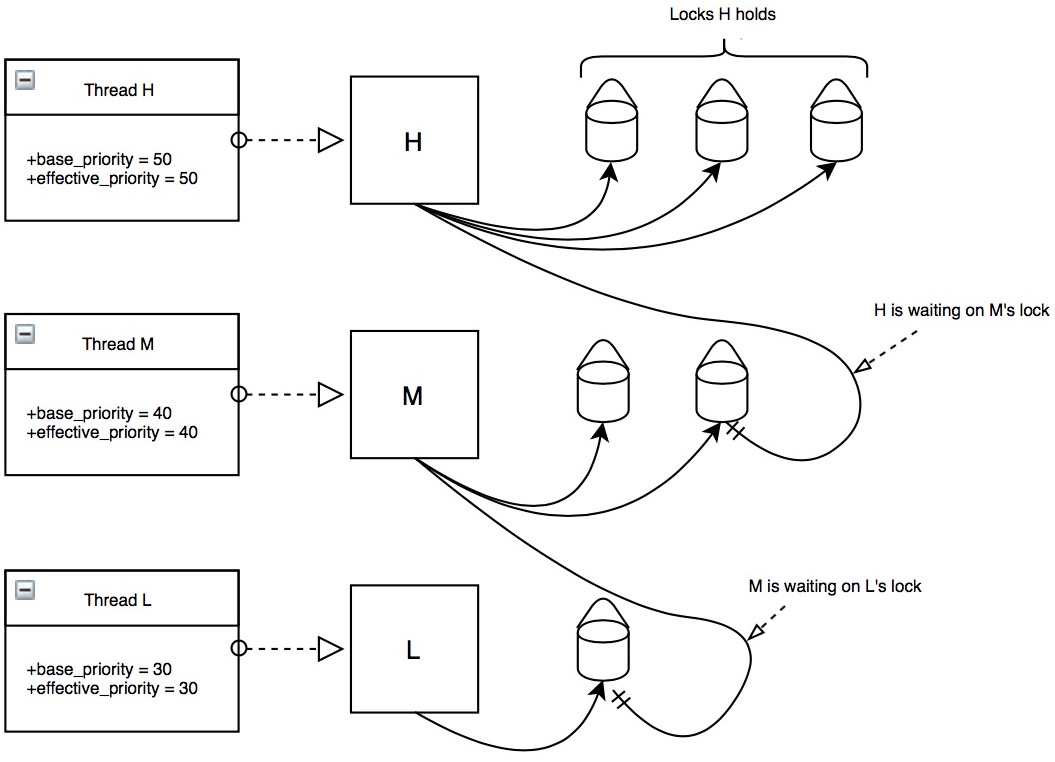
\includegraphics[width=0.6\textwidth]{Images/Task1/1Nested}
\caption{Initial State}
\end{figure}

In the following scenario (Figure 1), thread H is the highest priority thread and therefore in the running state. It currently has three locks, and wants to acquire a fourth by calling \texttt{lock\_acquire()}. If no thread owns the lock (i.e. \texttt{holder} is \texttt{NULL}), then H can acquire the lock. 

\begin{figure}[ht!]
\centering
\hspace{3em}
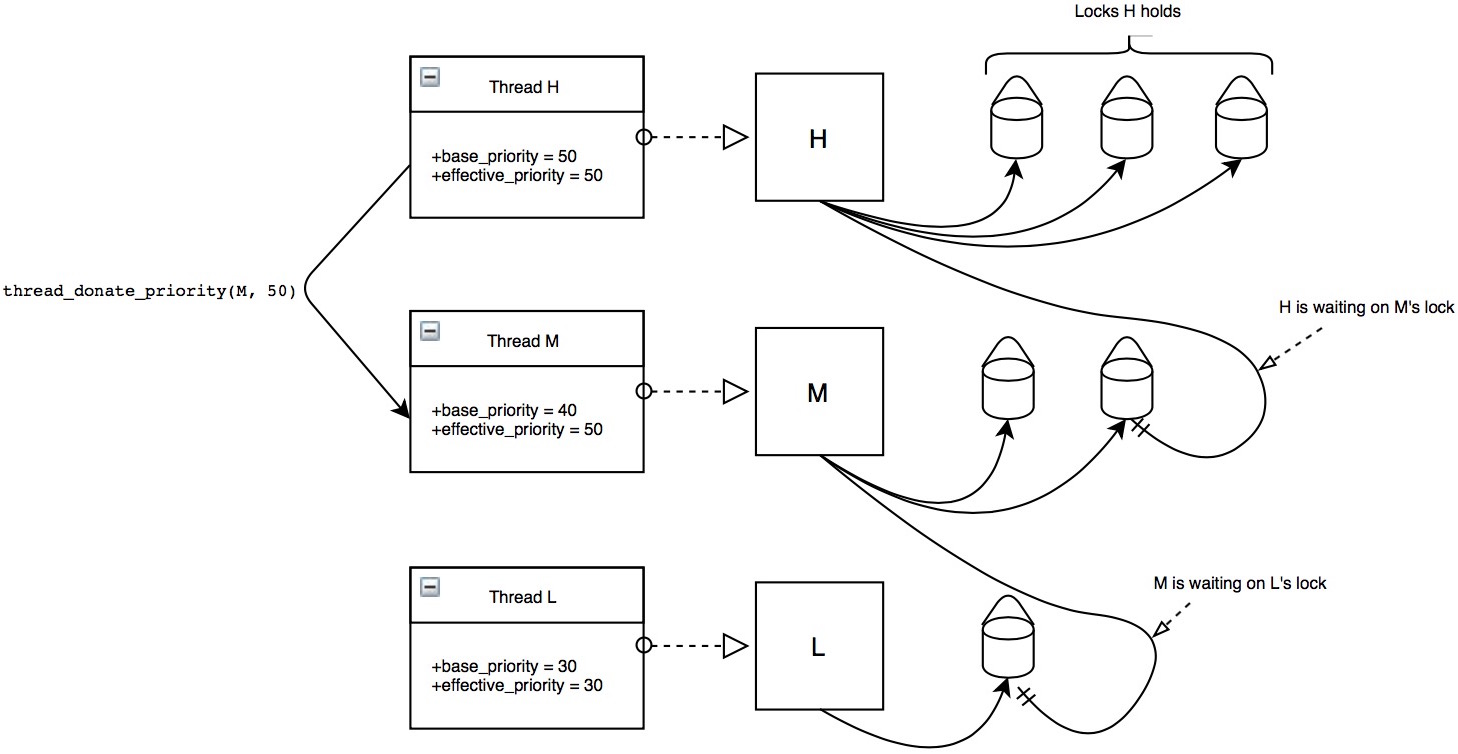
\includegraphics[width=0.8\textwidth]{Images/Task1/2Nested}
\caption{Second State}
\end{figure}

However, M has the lock, so H calls \texttt{thread\_donate\_priority(M, H->effective\_priority)} in Figure 2 so that M can release the lock, recalculate its priority, and H can continue to run. Unfortunately, it is the case that M itself is waiting on another lock L has, so M calls recursively \texttt{thread\_donate\_priority(L, M->effective\_priority)}, as shown in Figure 3.
\newpage

\begin{figure}[ht!]
\centering
\hspace{3em}
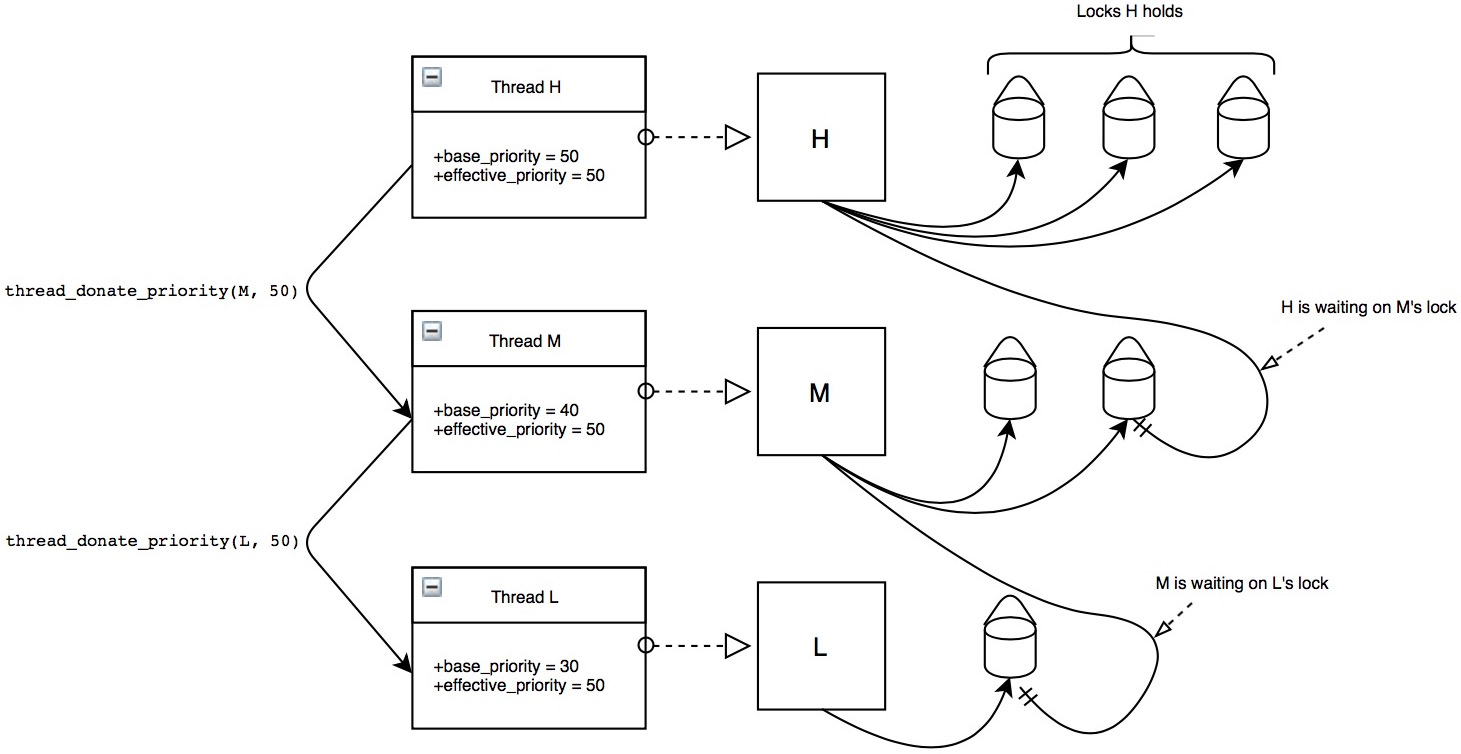
\includegraphics[width=0.8\textwidth]{Images/Task1/3Nested}
\caption{Third State}
\end{figure}

Now L has effective priority 50 and therefore runs. It checks if it is waiting on a lock through \texttt{waiting\_on\_lock}, (it isn't), so we have reached a base case, and \texttt{thread\_donate\_priority(L, M->effective\_priority)} simply returns. L continues to run, and releases the lock it's holding through \texttt{lock\_release()}. This in turn calls \texttt{thread\_recalculate\_priority(L)}, which checks the list of locks L holds \texttt{locks\_holding}. We iterate through all the locks L holds and see for each lock the list of waiting threads on that lock. The highest priority waiting thread would then set the effective priority of L to its effective priority. However, since L is not holding any locks, we simply set the effective priority to the base priority (Figure 4). 

\begin{figure}[ht!]
\centering
\hspace{3em}
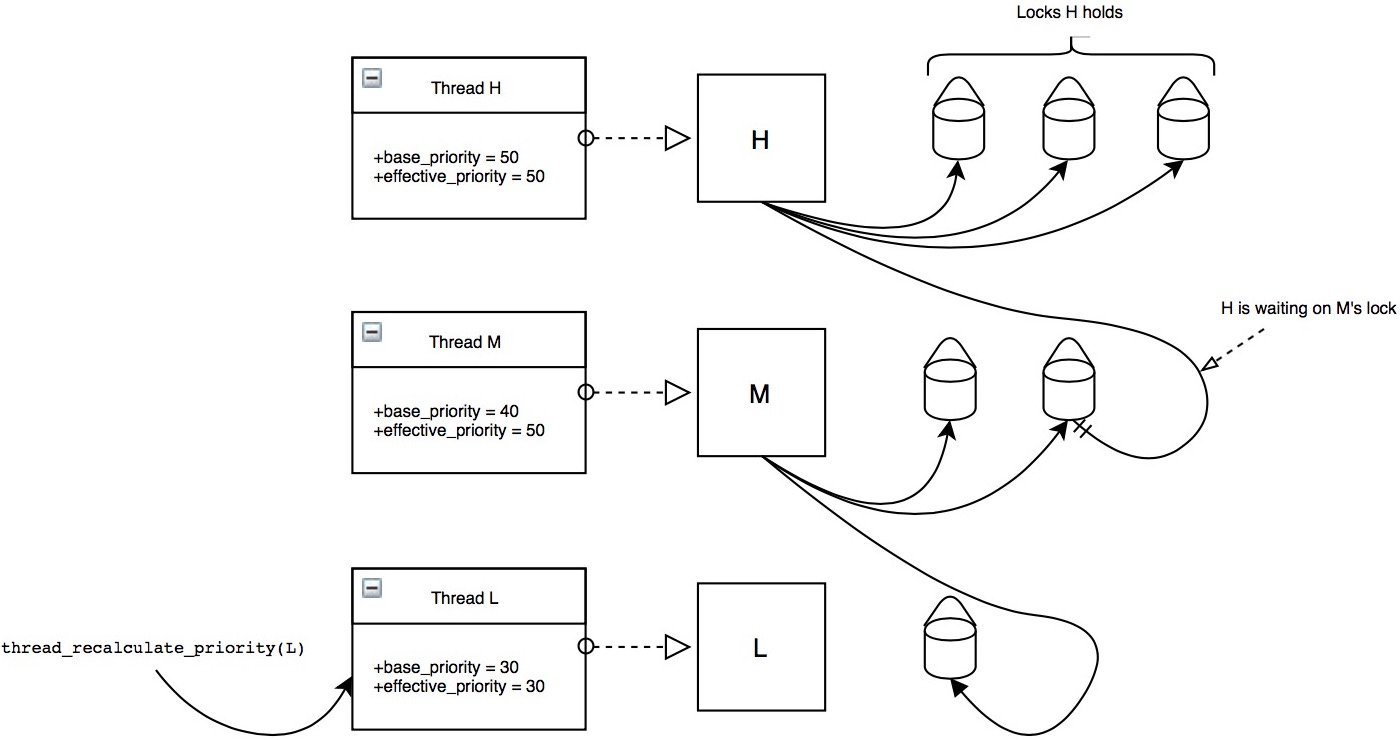
\includegraphics[width=0.8\textwidth]{Images/Task1/4Nested}
\caption{Fourth State}
\end{figure}

Note that in Figure 4 thread L has released the lock, and M is therefore not waiting on any more locks. It would therefore be unblocked and put in a running state. Since M is now running, it can release the lock H wants through \texttt{lock\_release()} which in turn calls \texttt{thread\_recalculate\_priority(M)}. We again iterate through all the locks M holds and see for each lock the list of waiting threads on that lock. The highest priority waiting thread would then set the effective priority of M to its effective priority. However, since M's list of locks have no waiters, we simply set the effective priority to the base priority (Figure 5). 

\begin{figure}[ht!]
\centering
\hspace{3em}
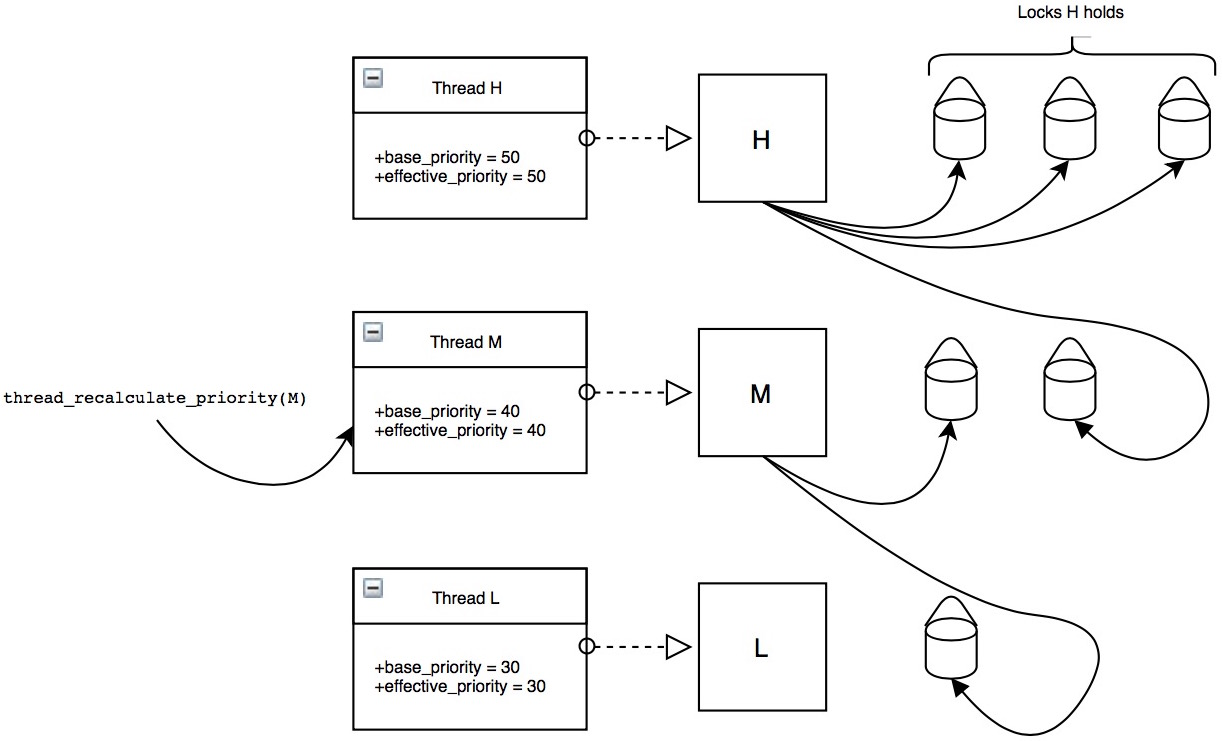
\includegraphics[width=0.8\textwidth]{Images/Task1/5Nested}
\caption{Fifth State}
\end{figure}

Again note how now M has released the lock and set back its effective priority.

\begin{figure}[ht!]
\centering
\hspace{3em}
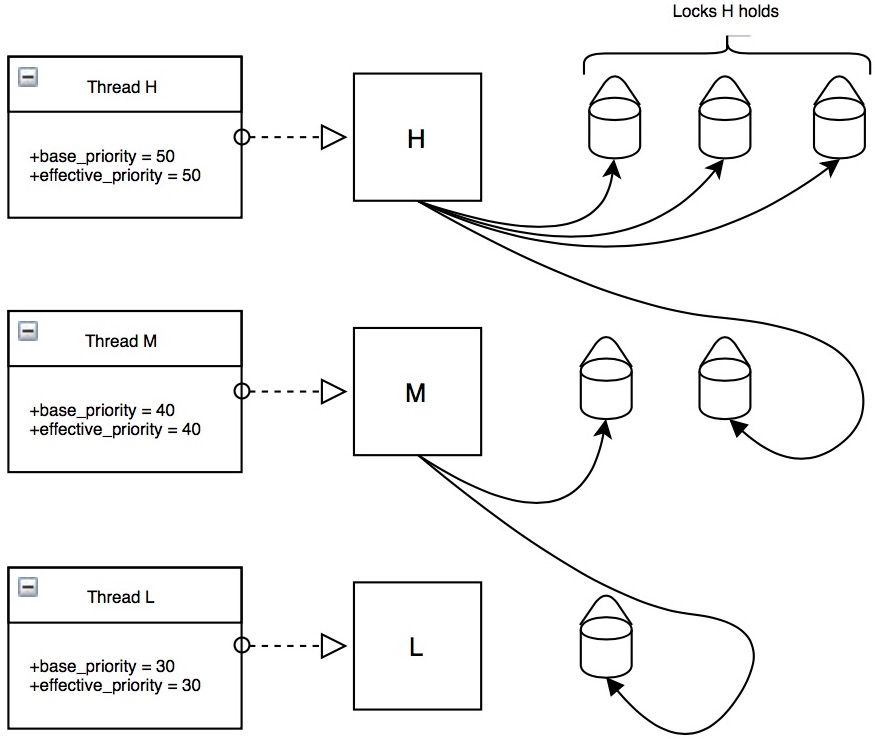
\includegraphics[width=0.6\textwidth]{Images/Task1/6Nested}
\caption{Final State}
\end{figure}

We thus reach our final state, avoiding starvation and deadlock.


%\begin{figure*}
%    \centering
%    \begin{subfigure}[b]{0.50\textwidth}
%   	    \hspace{2em}
%            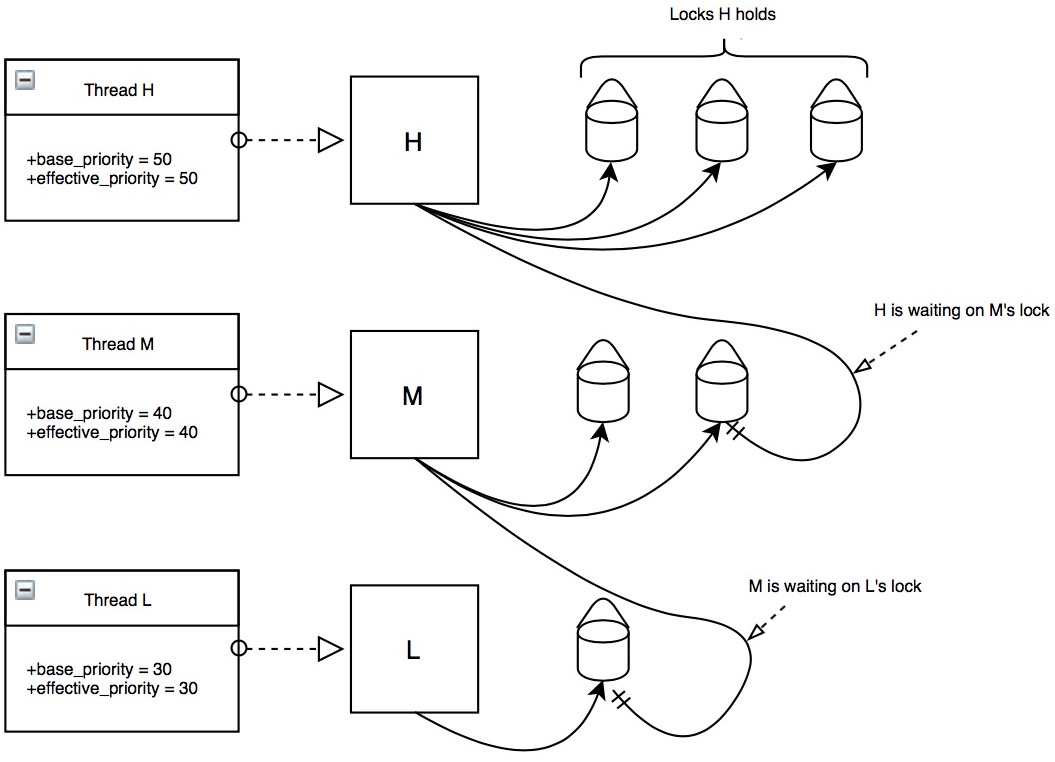
\includegraphics[width=\textwidth]{Images/Task1/1Nested}
%            \caption{Initial State}
%            \label{fig:a}
%    \end{subfigure}
%    
%    \begin{subfigure}[b]{0.49\textwidth}
%            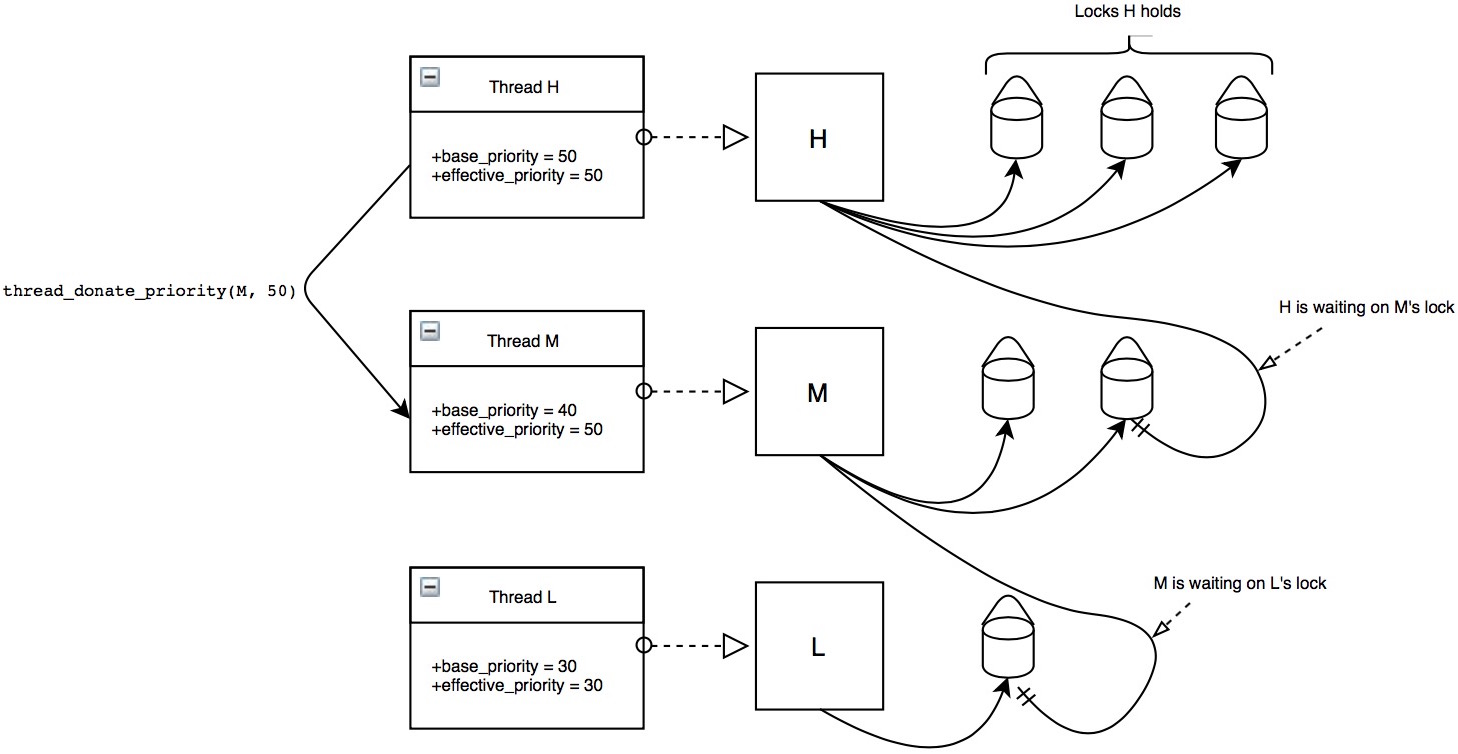
\includegraphics[width=\textwidth]{Images/Task1/2Nested}
%            \caption{c}
%            \label{fig:c}
%    \end{subfigure}
%    % ... this comment too
%    \begin{subfigure}[b]{0.49\textwidth}
%            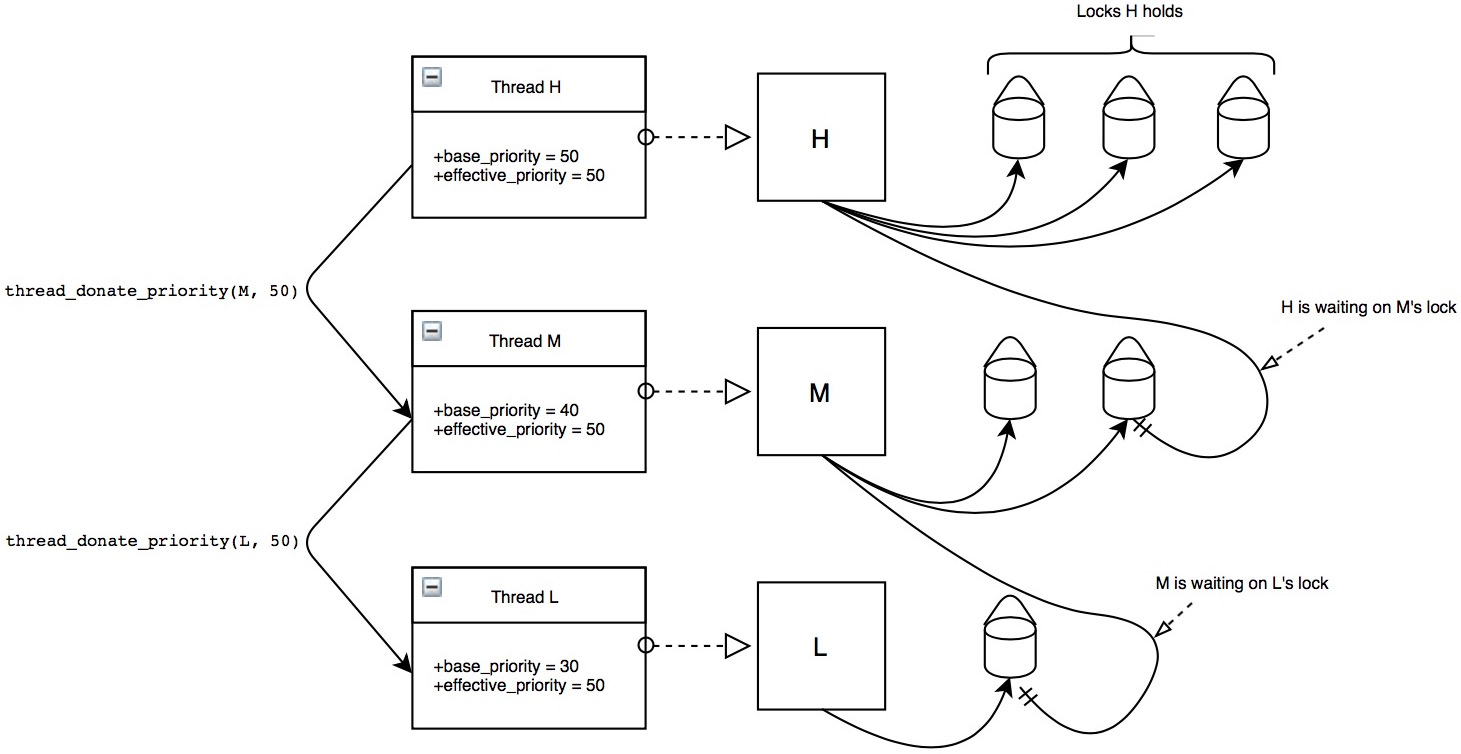
\includegraphics[width=\textwidth]{Images/Task1/3Nested}
%            \caption{d}
%            \label{fig:d}
%    \end{subfigure}
%    \begin{subfigure}[b]{0.49\textwidth}
%            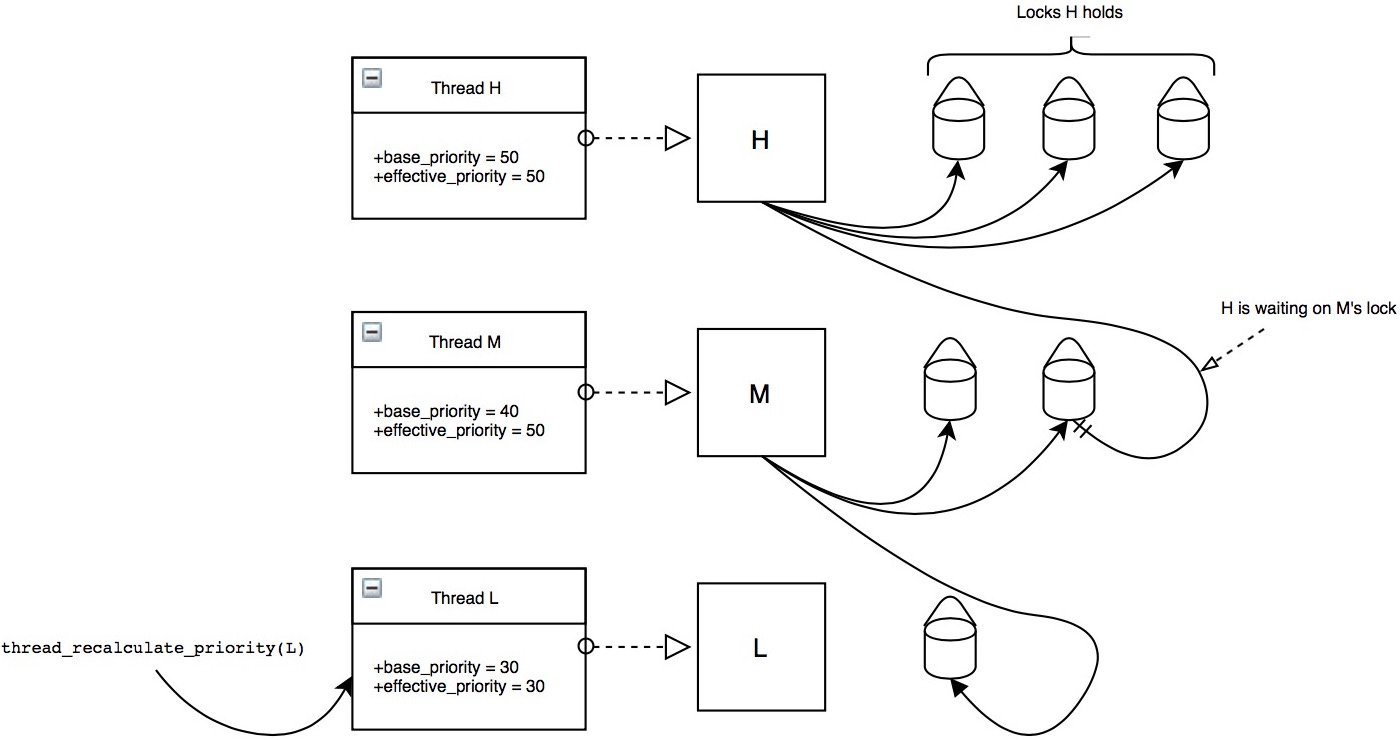
\includegraphics[width=\textwidth]{Images/Task1/4Nested}
%            \caption{c}
%            \label{fig:c}
%    \end{subfigure}
%    % ... this comment too
%    \begin{subfigure}[b]{0.49\textwidth}
%            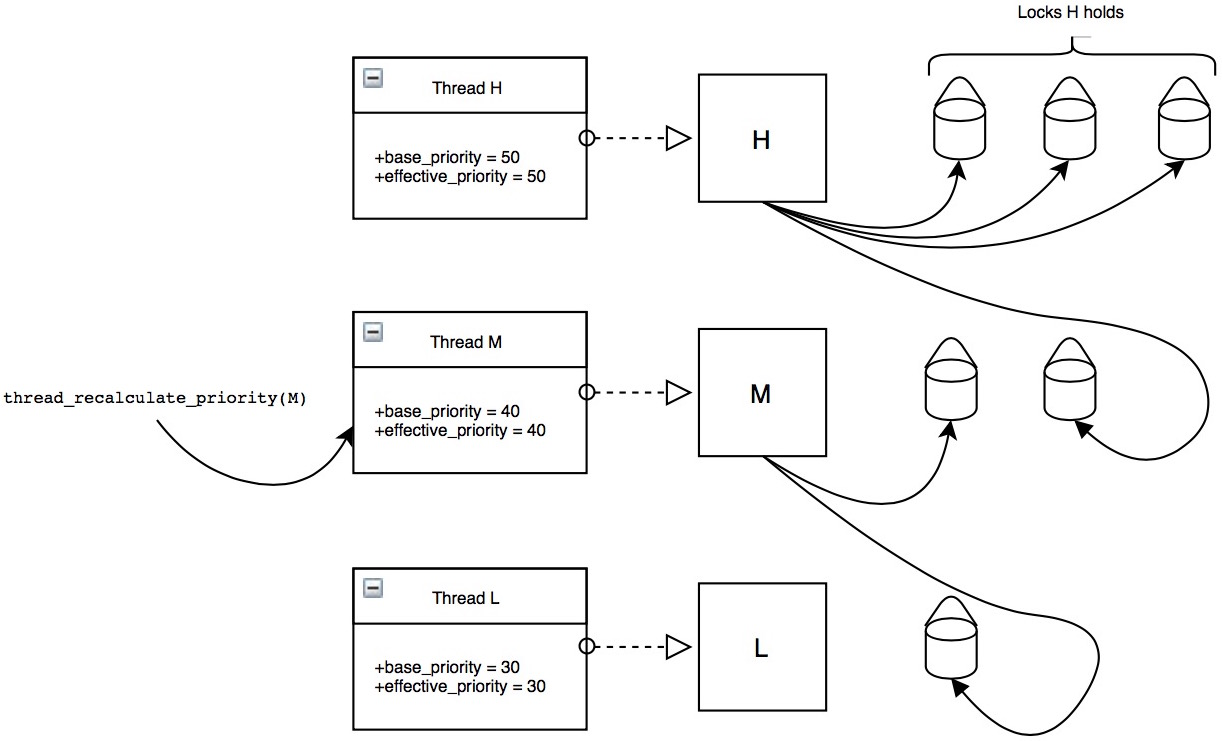
\includegraphics[width=\textwidth]{Images/Task1/5Nested}
%            \caption{d}
%            \label{fig:d}
%    \end{subfigure}
%     \begin{subfigure}[b]{0.50\textwidth}
%            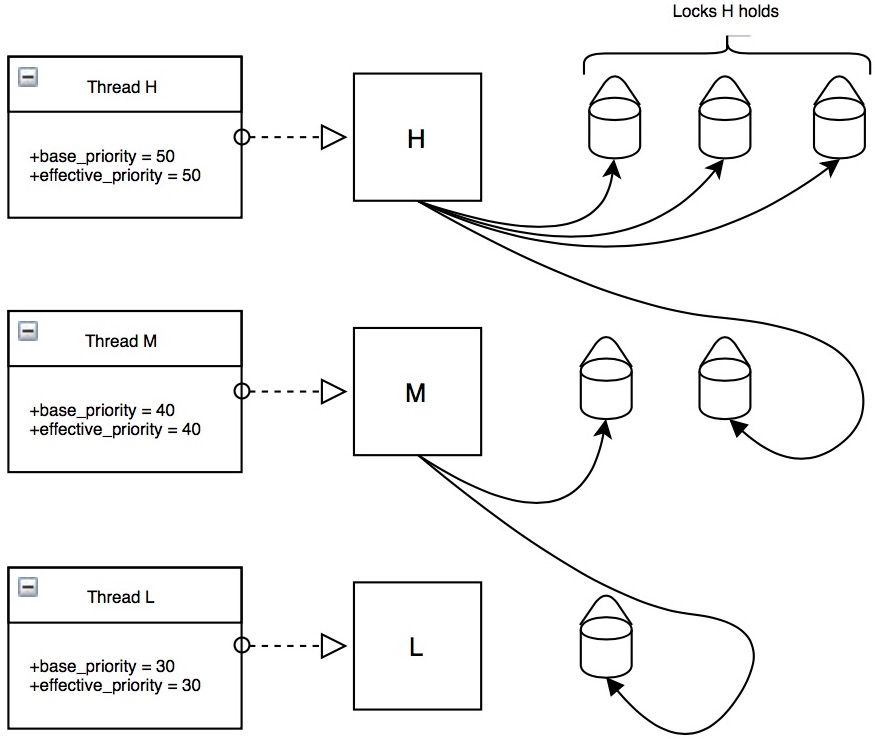
\includegraphics[width=\textwidth]{Images/Task1/6Nested}
%            \caption{Initial State}
%            \label{fig:a}
%    \end{subfigure}
%    \caption{Pictures of ABCD}\label{fig:ABCD}
%\end{figure*}


\subsection{Algorithms}
\subsubsection{Ensuring highest priority thread wakes up first}

To ensure that the highest priority thread waiting for a semaphore wakes up first, we use an ordered list of waiting threads,
in growing order of priority. When \texttt{sema\_down()} is called on a semaphore, the current thread is inserted into the list of waiting threads using the \texttt{less\_priority()} method which compares the priority of two threads. The thread is then blocked while it is waiting for \texttt{sema\_up()} to be called on the semaphore.

Once \texttt{sema\_up()} is called on the semaphore, the last thread in the list of waiting threads, which has the highest priority,
is woken up with \texttt{thread\_unblock()} and removed from the list of waiting threads.

Locks and condition variables both use a semaphore to block and wake up threads: therefore they will use their semaphore's 
ordered list of waiting threads as a way to ensure the highest priority thread will be woken up first, as explained above.

\subsubsection{Sequence of events in \texttt{lock\_acquire()}}

When a call to \texttt{lock\_acquire} causes a priority donation, the following sequence of events happens:

\begin{itemize}

\item If the lock doesn't have an owner, we simply acquire the lock, ensure that the current thread's \texttt{waiting\_on\_lock = NULL}, set the \texttt{lock\_holder} to be the current thread, and add the lock to the list of locks the thread owns.

\item If the lock already has a holder (a thread that is holding the lock), we use the helper method \texttt{thread\_donate\_priority()}, giving it as arguments the thread holding the lock as well as the current thread's priority.

\item If the thread holding the lock has a higher priority than the current thread, the holder continues holding the lock and we return from the method.

\item Otherwise, the current thread's priority becomes the holder's priority.

\item In that case, we check the holder's status: if it is blocked, we remove it from the list of waiting threads and reinsert it in the right order depending on its new priority. If the holder is ready to run, we remove it from the list of waiting threads and add it to the list of threads ready to run.

\item Finally, if the holder of the lock (Lock A) is waiting for another lock (Lock B) to be released, we call \texttt{thread\_donate\_priority()} with Lock B's holder and Lock A's holder's new priority: this helper method therefore works recursively in the case of nested priority donation. For a more detailed explanation on nested priorities, refer to question 1.1.2 with the nested priority diagrams.

\item We then leave the helper method, and call \texttt{sema\_down()} on the lock's semaphore.

\end{itemize}

\subsubsection{Sequence of events in \texttt{lock\_release()}}

When \texttt{lock\_release()} is called on a lock that a higher priority thread is waiting for, the following sequence of events happens:

\begin{itemize}

\item The lock's holder is set to NULL.

\item The lock is removed from the list of locks the current thread is holding.

\item We call a helper method \texttt{thread\_recalculate\_effective\_priority()} on the current thread: if the current thread does not hold any other locks, it takes back its base priority value and the method returns. Otherwise, it traverses through the list of locks it is holding, setting its effective priority to the largest effective priority out of the effective priorities of the lock's waiters.

\item In that case, if the current thread's effective priority is lower than the highest available priority found in the previous traversal, the thread yields.

\item Finally, we leave the helper method and \texttt{sema\_up()} is called on the lock's semaphore.

\end{itemize}

\subsection{Synchronization}
\subsubsection{Potential race in \texttt{thread\_set\_priority()}}

There are a few potential synchronization problems that could occur in \texttt{thread\_set\_priority()}, as well as in \texttt{thread\_donate\_priority()}, as these two functions are closely linked, because they both deal with the priorities of a thread. One problem that could occur is that \texttt{thread\_donate\_priority()} could be called within \texttt{thread\_set\_priority()} due to an interrupt causing another thread to run, just after we check to see if the newly set base priority is larger than the same thread's effective priority, but before setting the effective priority to equal the new base priority, which would happen in the if statement because the effective priority is the largest out of all donated priorities and the base priority. \texttt{thread\_donate\_priority()} being called here could change the thread's effective priority, but then the line of code inside the if statement would change the effective priority to be equal to the thread's base priority. The below code, from \texttt{thread\_set\_priority()}, is where the problem would occur:

\begin{lstlisting}
  struct thread *t = thread_current();

 /* Always sets the base priority to new_priority. */
  t->base_priority = new_priority;

  /* If base_priority is now larger than the threads effective priority,
     its effective priority can now be changed to be equal to the base
     priority, as effective priority is the maximum of base priority
     and donated priorities. */
  if (t->base_priority > t->effective_priority) {
	  t->effective_priority = t->base_priority;
  }
\end{lstlisting}

Also, if an interrupt occurs near the start of \texttt{thread\_donate\_priority()}, and then the base priority and effective priority of that thread get changed to be higher than the priority being donated, the effective priority will be immediately set to the donated priority, even though it has been modified.

This would happen if the interrupt occurs after we have checked whether the effective priority of the thread is larger than the donated priority, but before the effective priority is written to. Ideally, we would like the effective priority to not be modified by \texttt{thread\_set\_priority()} during \texttt{thread\_donate\_priority()}.

Both of these synchronization problems would be solved if \texttt{thread\_donate\_priority()} could not be called if \texttt{thread\_set\_priority()} has been called, but an interrupt has occurred before it finished executing, and vice versa. This means that a lock (or a semaphore initialised to 1) should be acquired (or downed) at the start of each of these functions, and released (or upped) at the end of each of these functions.

\subsection{Rationale: Choice of design}

One design we considered was giving each lock a priority, and allowing each lock to be donated to. The effective priority of a thread would therefore be the maximum priority of the locks it was holding and it's base priority. However, we decided to change this to a design where each thread holds a list of locks that it is holding, and each thread has a pointer to the lock that it is waiting on. This design makes a lot more sense, as locks do not actually have priorities, so it is easier to understand and modify. 

The list of locks being held by a thread makes it very easy to find the effective priority of a thread, as we can just traverse through the list, and find the maximum priority out of any threads waiting on any of these locks, and then comparing this to the thread's base priority. Also, the pointer to the lock that a thread is waiting on makes it a lot easier to donate priorities in a chain, where thread L donates to thread M, and thread M donates to thread H, for example. This is because when a tead is donated to, the lock it's waiting on can be recursively donated to, along the chain (after we check that whether \texttt{waiting\_on\_lock} is \texttt{NULL}).


\newpage

\section{Design Questions: Advanced Scheduler}
\subsection{Data Structures}
\subsubsection{Purpose of fixed-point macros and \texttt{typedef}}

Code from \texttt{fixed\_point.h}: 

\begin{lstlisting}
/* We are using a P.Q fixed-point format. P + Q must equal 31. */
#define P 17
#define Q 14
#define F (1 << (Q))

typedef int32_t fixed_point;

\end{lstlisting}

\texttt{P} and \texttt{Q} define the fixed-point format used (P.Q format) and \texttt{F} is used in the fixed-point arithmetic operations.

The typedef is used because a fixed-point number is represented as a 32-bit signed int, in P.Q format, where by default \texttt{P = 17}, and \texttt{Q = 14}. Needed for some of the data values stored and calculated for mlfqs mode, as floating-point arithmetic would slow the kernel.

\subsubsection{Purpose of mlfqs specific data structures}

\begin{enumerate}

\item From thread.c: 
\begin{lstlisting}
/* Array of ready_lists depending on priority for BSD Scheduler */
static struct list ready_lists_bsd[NUM_PRIORITIES];
static struct list ready_list;

/* Simply the number of threads in ready_lists_bsd.
   Needed to calculate load_avg. Only used in mlfqs mode. */
static int num_of_ready_threads;

\end{lstlisting}


\item From thread.h:
\begin{lstlisting}
/* Number of priorities in Pintos. Used for the BSD Scheduler. */
#define NUM_PRIORITIES (PRI_MAX - PRI_MIN + 1)

/* BSD scheduler priority scaling factors */
/* priority calculation includes "- recent_cpu / RECENTCPU_DIVISOR"... */
#define RECENTCPU_DIVISOR 4
/* ...and "-nice*NICE_COEFFICIENT" */
#define NICE_COEFFICIENT 2
/* These are fixed_point coefficients for load_avg calculation. */
#define LOAD_AVG_COEFFICIENT DIV_FIXED_POINT_BY_INT(TO_FIXED_POINT(59), 60)
#define READY_THREAD_COUNT_COEFFICIENT       \
                              DIV_FIXED_POINT_BY_INT(TO_FIXED_POINT(1), 60)
                              
\end{lstlisting}

\newpage

\item From thread.h:
\begin{lstlisting}
struct thread
  {
        .
        .
    int effective_priority;          /* Used in both default and mlfqs mode. */
        .
        .
    int nice;                          /* Thread niceness value */
    fixed_point recent_cpu;            /* CPU time recently received */
        .
        .
  };
  
\end{lstlisting}

\item From thread.h:
\begin{lstlisting}
fixed_point load_avg;                  /* System-wide load_avg variable. */

\end{lstlisting}

\end{enumerate}

\begin{enumerate}

\item \texttt{ready\_lists\_bsd} is the mlfqs version of \texttt{ready\_list}. It is an array holding all ready queues for the BSD scheduler. Index into the array corresponds to the priority of the queue (Index 0 is \texttt{PRI\_MIN}, index 1 is \texttt{PRI\_MIN + 1}, etc.). \texttt{num\_of\_ready\_threads} is only used in mlfqs mode. It is the number of threads in \texttt{ready\_lists\_bsd}, and is needed to recalculate \texttt{load\_avg}.

\item \texttt{NUM\_PRIORITIES} is used when defining and traversing \texttt{ready\_lists\_bsd}. This means \texttt{PRI\_MIN} and \texttt{PRI\_MAX} could be changed, and our mlfqs implementation would still work. \texttt{RECENTCPU\_DIVISOR} and \texttt{NICE\_COEFFICIENT} are used in the formula for recalculating \texttt{priority} in mlfqs mode. The macros \texttt{LOAD\_AVG\_COEFFICIENT} and \texttt{READY\_THREAD\_COUNT\_COEFFICIENT} are used in the formula for recalculating \texttt{priority} in mlfqs mode. These all get rid of magic numbers.

\item We added two members to \texttt{struct thread} for this part of task 2 - \texttt{nice} and \texttt{recent\_cpu}. In mlfqs mode, each thread has a 'niceness' value - it determines how 'nice' the thread is to other threads, and so affects it's threads priority. Each thread also has a \texttt{recent\_cpu}, which measures the amount of CPU time a thread has received recently. To store the \texttt{priority} of a thread in mlfqs mode, we re-used \texttt{effective\_priority} from the first part of this task.

\item \texttt{load\_avg} is a system-wide OS data value, which estimates the average number of threads ready to run over the past minute.

\end{enumerate}

\subsection{Algorithms}
\subsubsection{Table}

If we have three threads A, B and C with \texttt{nice} values 0, 1 and 2, and \texttt{recent\_cpu} values equal to 0, the following scheduling decisions will be made:

\newpage

\begin{table}[]
\centering	 
\caption{Thread Scheduling Decisions}	 
\label{Thread table}	 
\begin{tabular}{|l|l|l|l|l|l|l|l|}	 
\hline 
\multirow{2}{*}{\textbf{\begin{tabular}[c]{@{}l@{}}Timer \\ ticks\end{tabular}}} & \multicolumn{3}{l|}{\textbf{Recent cpu}} & \multicolumn{3}{l|}{\textbf{Priority}} & \multirow{2}{*}{\textbf{\begin{tabular}[c]{@{}l@{}}Thread\\ to run\end{tabular}}} \\ \cline{2-7} 
                                                                               & \textbf{A}   & \textbf{B}   & \textbf{C}  & \textbf{A}  & \textbf{B}  & \textbf{C} &                                                                                   \\ \hline 
\textit{0}                                                                       & 0            & 0            & 0           & 63          & 61          & 59         & A                                                                                 \\ \hline	 
\textit{4}                                                                       & 4            & 0            & 0           & 62          & 61          & 59         & A                                                                                 \\ \hline	 
\textit{8}                                                                       & 8            & 0            & 0           & 61          & 61          & 59         & B                                                                                 \\ \hline	 
\textit{12}                                                                      & 8            & 4            & 0           & 61          & 60          & 59         & A                                                                                 \\ \hline 
\textit{16}                                                                      & 12           & 4            & 0           & 60          & 60          & 59         & B                                                                                 \\ \hline	 
\textit{20}                                                                      & 12           & 8            & 0           & 60          & 59          & 59         & A                                                                                 \\ \hline	 
\textit{24}                                                                      & 16           & 8            & 0           & 59          & 59          & 59         & C                                                                                 \\ \hline 
\textit{28}                                                                      & 16           & 8            & 4           & 59          & 59          & 58         & B                                                                                 \\ \hline	 
\textit{32}                                                                      & 16           & 12           & 4           & 59          & 58          & 58         & A                                                                                 \\ \hline 
\textit{36}                                                                      & 20           & 12           & 4           & 58          & 58          & 58         & C                                                                                 \\ \hline 
\end{tabular}	 
\end{table}


\subsubsection{Ambiguities in scheduler specification and resolution}

The choice of which thread to run when multiple threads have the same priority is ambiguous. However the specification explains we should switch through the threads in 'round robin' order which means that when multiple threads have the same priority, the one which has been waiting for the longest should run. We have implemented this in our scheduler by pushing threads to the front of our ordered list of ready threads for a certain priority, and popping the back of the list when we take a ready thread and make it run. This simulates the behaviour of a queue: the first thread to enter the priority queue will be the first one removed from the list and added to the list of threads that are ready to run. 

\subsubsection{Dividing cost of scheduling}


We have tried to put as little code as possible inside the interrupt context to improve efficiency and precision. Indeed, as an interrupt happens often (every 0.04 seconds), we do not want to recompute values if we do not need to as we will spend too much time inside the interrupt context and we will lose speed. Putting the code outside the interrupt context as much as possible allows the code only to be used when it is needed, therefore keeping the code efficiency as high as possible. 


\subsection{Rationale}
\subsubsection{Critique of design}

We put the code to deal with updating the data values such as \texttt{recent\_cpu} in \texttt{thread\_tick()} rather than in \texttt{timer\_interrupt()}, as the code to update these values should all be contained within \texttt{thread.c}, and provides a better level of abstraction. A disadvantage with out design is that we implemented our mlfqs version of \texttt{ready\_list} - \texttt{ready\_lists\_bsd}, using a static array of queues (\texttt{struct list}s), with one queue for each possible priority. This took a long time to traverse, involving a lot of checking to see if a queue is empty or not. A better design would have involved using a single list, and sorting it based on the priorities of the threads, as it would most likely take less time to traverse.

 An advantage to our design was that we made a function called \texttt{add\_to\_ready\_list()}, which adds a thread to the appropriate list of ready threads in both mlfqs mode and non-mlfqs mode. This meant that we didn't need lots of if statements dotted around our files whenever we wanted to add a thread to the ready list (These if statements would require us to check \texttt{bool thread\_mlfqs} and then add to the appropriate ready list). Also, the index of a queue in \texttt{ready\_lists\_bsd} corresponds to its priority, which made it a lot easier to find a queue with a specific priority, and looks a lot neater. 

Instead of dealing with \texttt{PRI\_MAX} and \texttt{PRI\_MIN}, we made a macro \texttt{define NUM\_PRIORITIES (PRI\_MIN - PRI\_MAX + 1)} to be used mostly when creating and traversing \texttt{ready\_lists\_bsd}, so that \texttt{PRI\_MAX} and \texttt{PRI\_MIN} can be changed, but our implementation will still work - we don't depend on \texttt{PRI\_MAX} being 63 and \texttt{PRI\_MIN} being 0. Another advantage is that we have a \texttt{num\_of\_ready\_threads} static variable in \texttt{thread.c}, which gets incremented and decremented when necessary, which is a better design than having a function to calculate the number of ready threads when we needed the value (to calculate \texttt{load\_avg}), which would have to traverse all of \texttt{ready\_lists\_bsd}. 

Finally, a disadvantage to our design is that we re-used the \texttt{effective\_priority} member in \texttt{struct thread} for the priority data value in the advanced scheduler. This is harder to read and understand. However, it allows some functions to behave in exactly the same way during mlfqs mode and non-mlfqs mode, when the priority/effective priority has to be accessed.

\subsubsection{Design in fixed-point arithmetic}

We decided to implement fixed-point arithmetic using macros defined in a separate file. The macros for \texttt{P} and \texttt{Q} lets the P.Q format we use for fixed-point numbers be easily tweaked. By default, this is a 17.14 fixed-point format, which represents a maximum value of $(2^{31} - 1)/2^{14} = 131,071.999$, so this should be sufficient. The other macros are to do the actual fixed-point operations. 

We decided to use macros instead of functions because these operations need to be carried out many times per second, to update the data values required for the advanced scheduler, and function calls would make these operations take too much time. As well as this, the macros still kept the readability of a function call, with the only disadvantage being that there is no type-checking for macros. However, in the arguments for a macro, \texttt{n} is always used to represent an \texttt{int}, and \texttt{x} or \texttt{y} is always used to represent a \texttt{fixed\_point}. To make all fixed-point arithmetic clearer, we used \texttt{typedef int32\_t fixed\_point}, so that it is clear when you are using a fixed-point number, and avoids confusion.


%----------------------------------------------------------------------------------------

\end{document}
